\pgfplotsset{
  every axis plot/.append style={
    line width=3pt
  }
}

\begin{table}[H]
  \centering
  \caption{Нелинейные активационные функции}\label{actvs}
  \begin{tabular}{|c|c|c|}
    \hline    
    \hyperlink{name}{Название} & \hyperlink{func}{Функция} & \hyperlink{chart}{Вид}\\
    \hline
    Сигмоидная &  \resizebox{0.2\hsize}{!}{$\sigma(x)=\frac{1}{1+e^{-x}}$}
    & 
    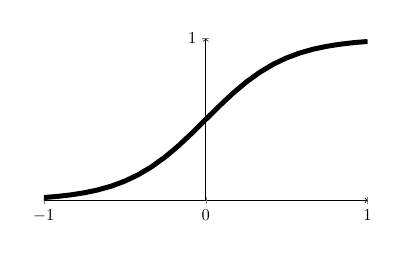
\begin{tikzpicture}[baseline={(0,0.8)}, scale=0.6]      
      \begin{axis}[
        axis equal image,
        axis lines=middle,
        axis line style={->},
        x label style={at={(axis description cs:0.5,-0.1)},anchor=north},
        y label style={at={(axis description cs:-0.1,.5)},rotate=90,      anchor=south},
        extra x ticks=0,
        % extra y ticks=1,
        ymin=0,ymax=1,
        ytick={0, 1},
        xtick={-1, 0, 1}
        ]
        \addplot[domain=-1:1, variable=\x] ({\x},{1/(1+exp(-4*\x))});
      \end{axis}      
    \end{tikzpicture}
   
    \\
    \hline
    Гиперболический тангенс 
    &
    \resizebox{0.2\hsize}{!}{$f(x)=\frac{e^x-e^{-x}}{e^z+e^{-z}}$}
    & 
    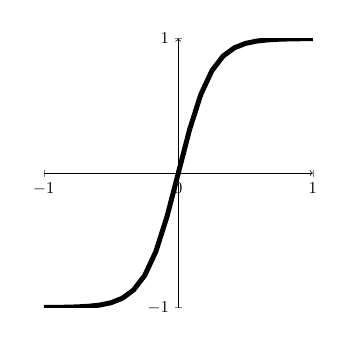
\begin{tikzpicture}[baseline={(0,1.5)},scale=0.6]
      \begin{axis}[
        axis equal image,
        axis lines=middle,
        axis line style={->},
        x label style={at={(axis description cs:0.5,-0.1)},anchor=north},
        y label style={at={(axis description cs:-0.1,.5)},rotate=90,      anchor=south},
         extra x ticks=0,  
        % extra y ticks=1,
        ymin=-1,ymax=1,
        ytick={-1, 0, 1},
        xtick={-1, 0, 1}
        ]
        \addplot[domain=-1:1, variable=\x]({\x},{tanh(4*\x)});
      \end{axis}      
    \end{tikzpicture} 
    \\
    \hline
    ReLU & \resizebox{0.2\hsize}{!}{$f(x) =\begin{cases}
    0, & x<0 \\ 
    x, & x \geq 0.
    \end{cases}$} & 
    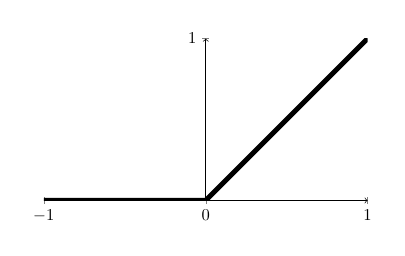
\begin{tikzpicture}[baseline={(0,0.8)},scale=0.6]
      \begin{axis}[
        axis equal image,
        axis lines=middle,
        axis line style={->},
        x label style={at={(axis description cs:0.5,-0.1)},anchor=north},
        y label style={at={(axis description cs:-0.1,.5)},rotate=90,anchor=south},
         extra x ticks=0,  
        % extra y ticks=1,
        ymin=0,ymax=1,
        ytick={0, 1},
        xtick={-1, 0, 1}
        ]
        \addplot[domain=-1:1, variable=\x]({\x},{ifthenelse(\x<0,0,\x)});
      \end{axis}      
    \end{tikzpicture}
    \\          
    \hline            
  \end{tabular}
\end{table}